\section{The IceCube in-ice Array and DeepCore}

The IceCube Neutrino Observatory consists of the so-called \emph{in-ice} array, optimized for astrophysical neutrino observations, the \emph{DeepCore} array, used primarily for the observation of atmospheric neutrinos, and the \emph{IceTop} surface array that can be used to study air showers from cosmic rays.

\subsection{The Antarctic Ice}

The detection medium of the IceCube detector is the Antarctic glacier that has formed from layers of snow being deposited top of each other over the course the past $\sim\num{100000}$ years\todo{reference}.
The weight of the upper layers compresses the lower layers into a dense, crystalline structure.
As a result, the optical properties of the ice change mostly in the direction perpendicular to the layers, forming a geological record of the atmospheric conditions of the Earth.
The transmission of light through the ice is primarily characterized by the scattering and absorption length. Within the volume of IceCube, scattering lengths vary between \SI{20}{\meter} and \SI{100}{\meter}, while absorption lengths range from \SI{100}{\meter} to \SI{400}{\meter}. Both quantities are highly correlated, such that the absorption length is approximately four times as large as the scattering length.\todo{cite ice model?}
This stratigraphy was traced at millimeter resolution using a laser dust logger deployed down seven IceCube drill holes as described by \cite{dustlogger}.
The most notable feature of the stratigraphy is the \emph{dust layer} at depths between 2000~m and 2100~m as shown in \reffig{icecube-schematic}.
The optical properties of the ice within the dust layer are particularly poor.
The ice below the dust layer where the DeepCore fiducial volume is located has the best optical properties of the entire IceCube volume.

\subsection{In-Ice Array}
The 5160 Digital Optical Modules (DOMs) that make up the IceCube in-ice array are distributed over 86 strings.
Of these, 78 are arranged on a hexagonal grid spanning an area of approximately one square-kilometer with a horizontal spacing of $\sim$150~m with respect to their closest neighboring strings\sidecite{icecube_detector_17}. Each of these strings holds 60 DOMs at depths between 1450~m and 2450~m with a 17~m vertical spacing.
The volume and instrumentation density of this array is optimized for astrophysical neutrinos that are found at energies above 1~TeV\cite{icecube_detector_17}.
The electric signals measured in each DOM are digitized  and sent to the \emph{IceCube lab (ICL)}, where the signal is processed, compressed, and sent North via satellite for offline processing.
\reffig{ic_detector} gives an overview of the detector including the IceCube Lab, the ice surface and the bedrock, and a schematic of the layout of the strings is shown in \reffig{icecube-schematic}.

\begin{figure}
	\centering 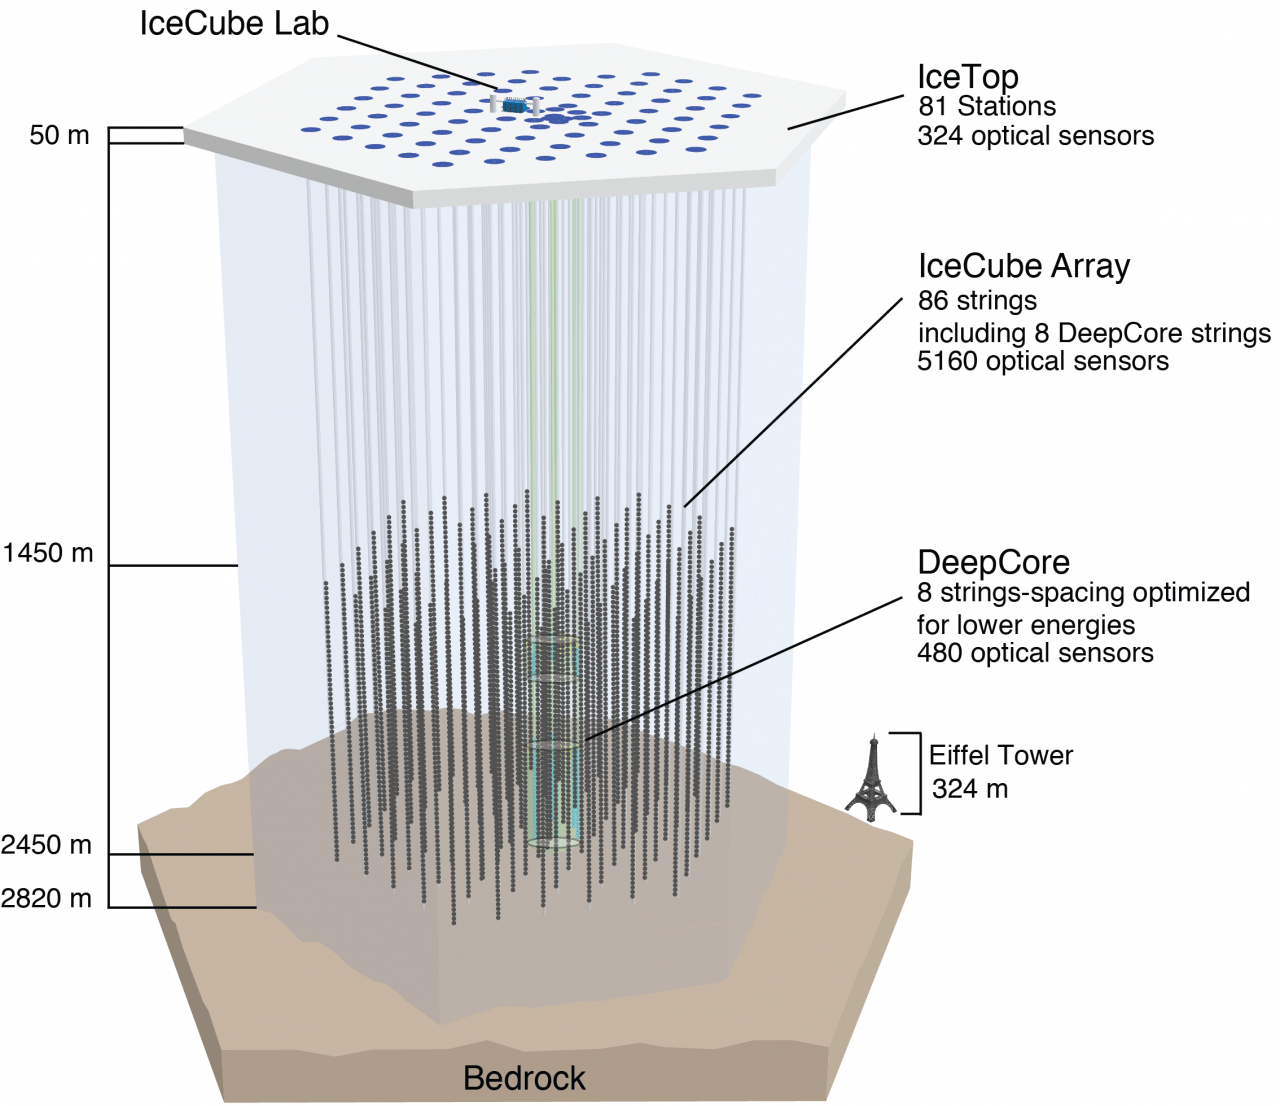
\includegraphics{figures/icecube/IceCubeArray_slim.png}
	\caption{An overview of the IceCube detector}
	\label{fig:ic_detector}
\end{figure}

\subsubsection{DeepCore}
The remaining 8 strings that are not part of the hexagonal grid are located near the center of the IceCube detector and form the \emph{DeepCore} sub-array\sidecite{DeepCore}.
The DOMs on the DeepCore strings have a higher quantum efficiency than those in the rest of the detector and are placed more closely together to lower the minimum energy threshold for neutrino observations to a few GeV.
Of the 60 DOMs on each DeepCore string, 50 are placed at depths between 2100~m and 2500~m, where the ice is the most transparent compared to the rest of the IceCube's volume (see also the side band in the bottom panel of Figure~\ref{fig:icecube-schematic}).
Together with 7 strings from the in-ice array, the DeepCore strings instrument the DeepCore 20~MT \emph{fiducial volume} as shown in the upper panel of Figure~\ref{fig:icecube-schematic}.
The remaining 10 DOMs are located at depths between 1750~m and 1850~m and are used as a veto cap to reject atmospheric muons entering the detector directly from above.
In addition, the larger hexagonal IceCube array also serves as a veto for observations inside the DeepCore fiducial volume.
\begin{figure}
    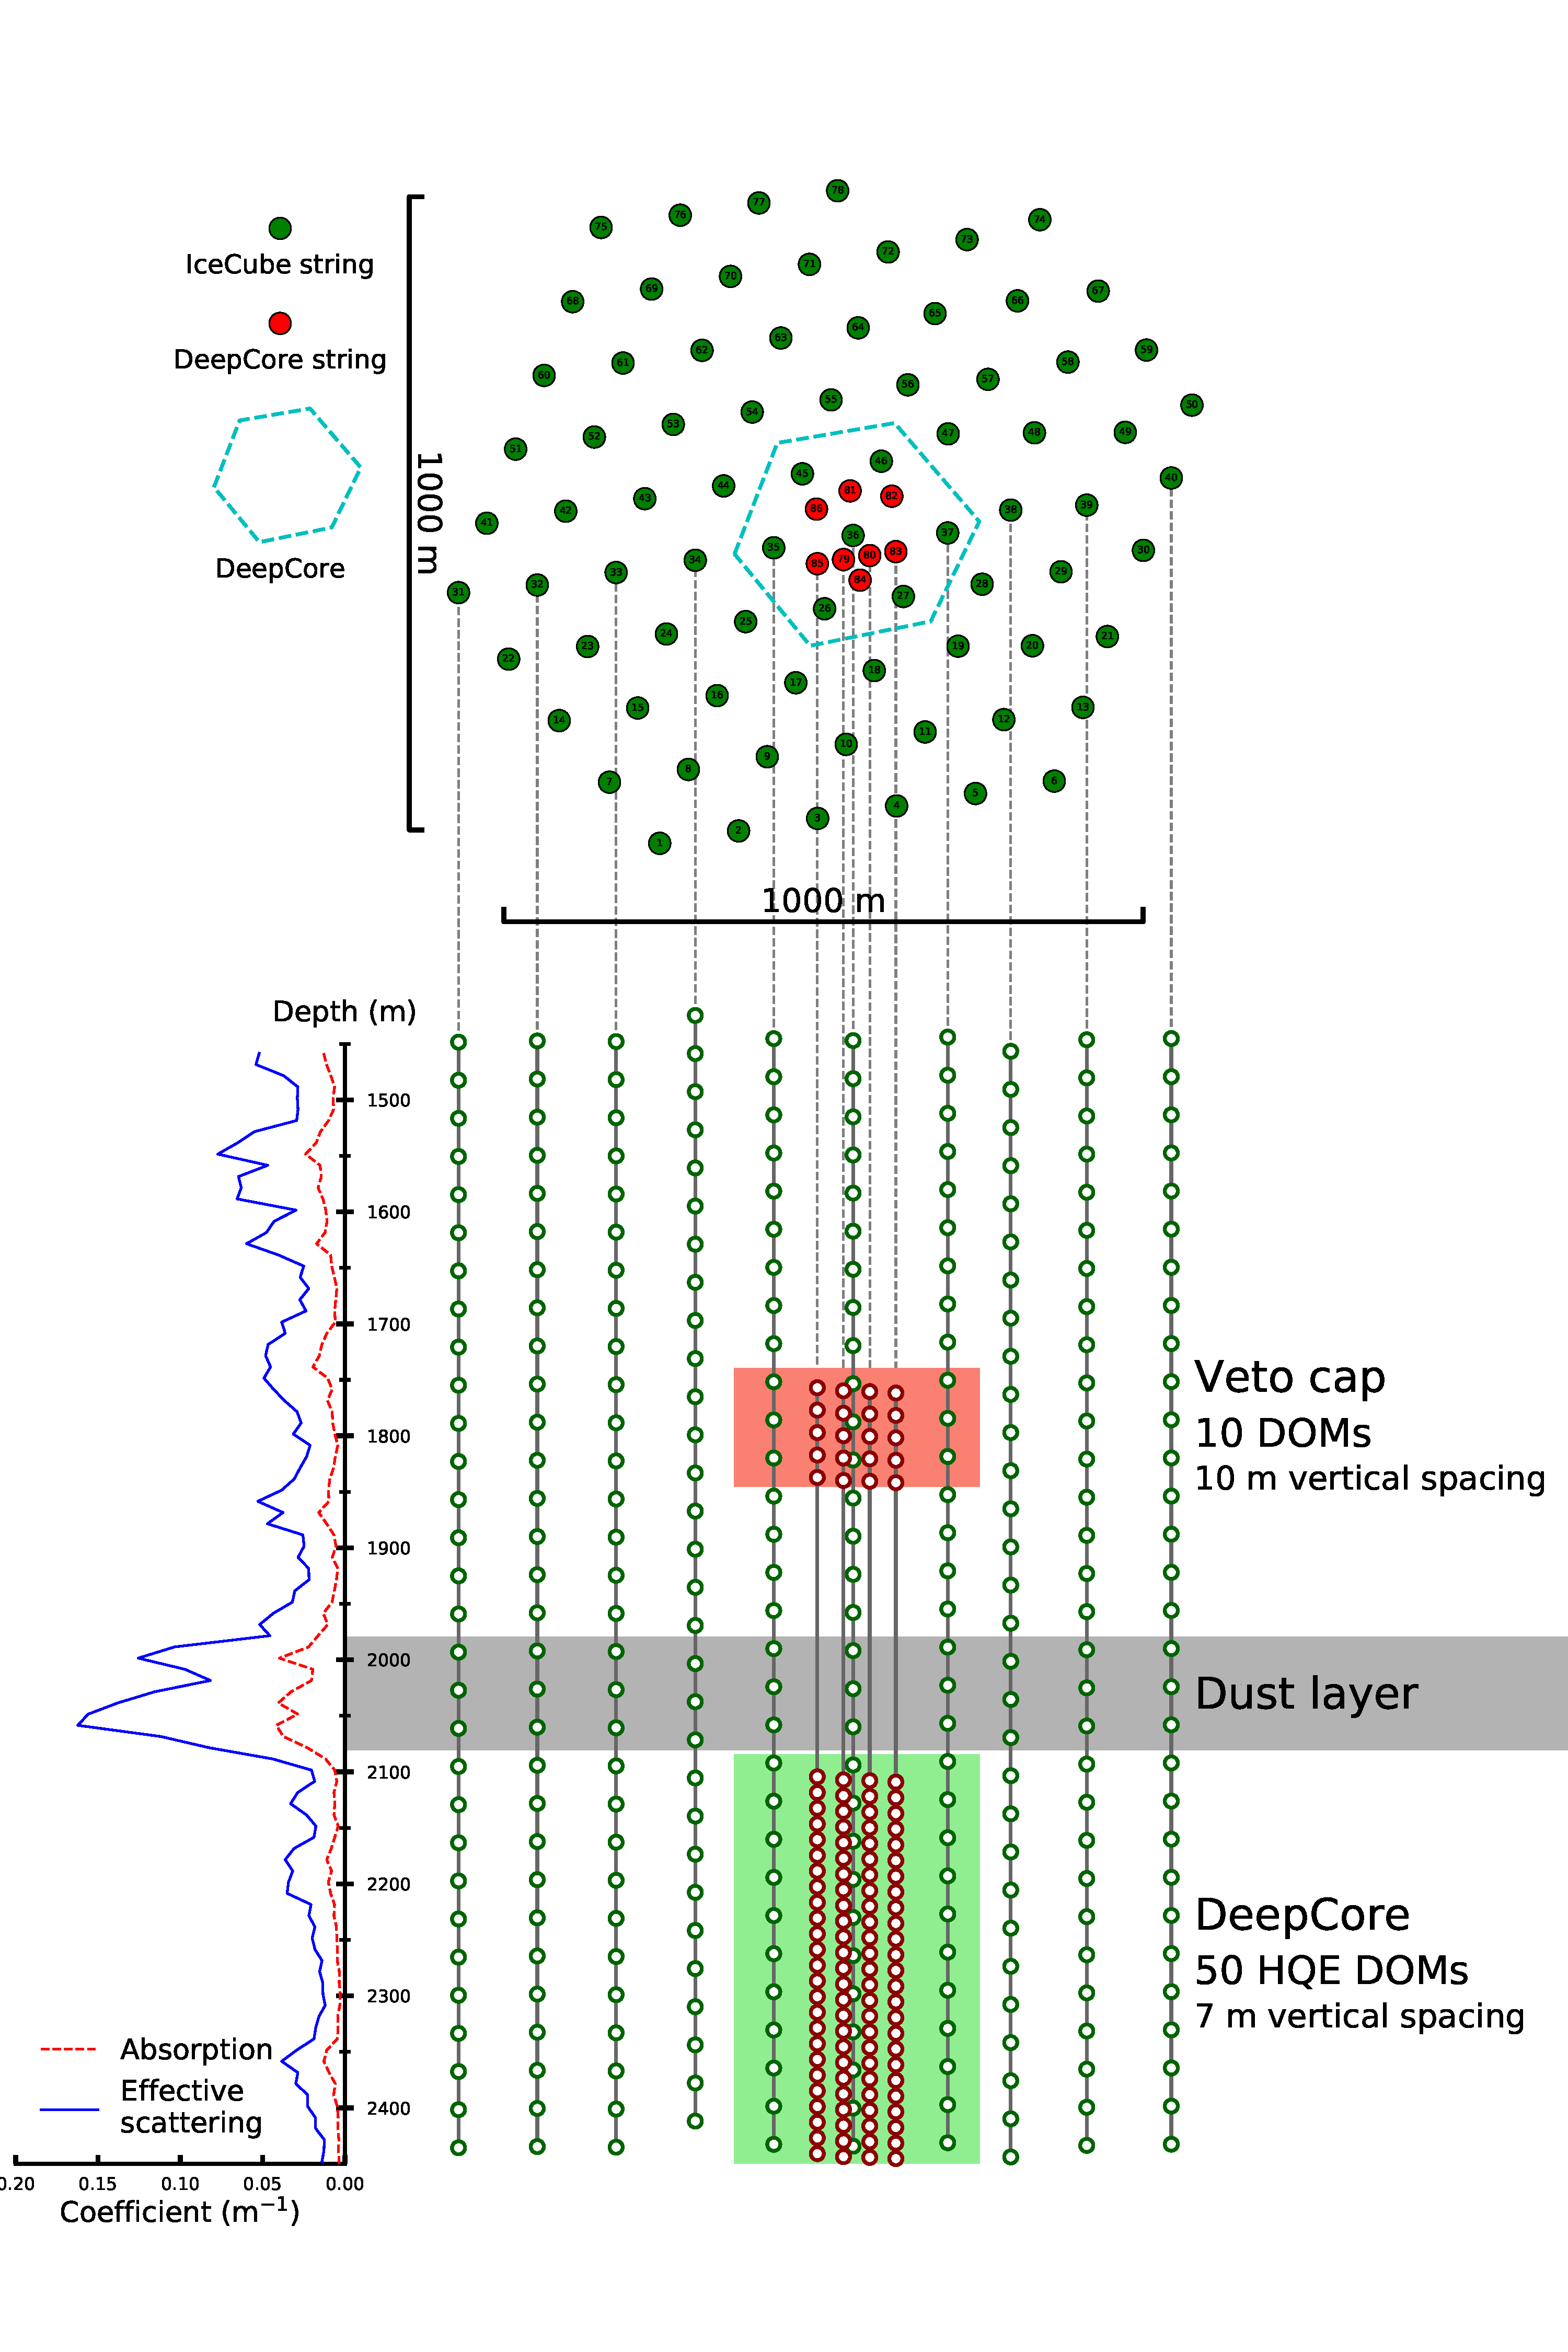
\includegraphics[width=0.9\linewidth]{figures/icecube/DeepCore_geometry.pdf}
    \caption{Schematic view of the IceCube detector as seen from the top (upper panel) and the side(lower panel). The DeepCore fiducial volume is indicated by the hexagon in the upper panel and the green shaded area in the bottom panel. The side-band on the lower panel shows the scattering and absorption coefficients as a function of depth.}
    \label{fig:icecube-schematic}
\end{figure}

\subsection{IceTop}

In addition to the in-ice array, IceCube also contains a surface array called \emph{IceTop}, consisting of 81 stations spread across an area of 1~km$^2$ that is used to detect muons from air showers.
It is typically used as a veto against atmospheric muons, but also functions as a detector in its own right measuring the spectrum and composition of cosmic particles.
%TODO: citation
However, it is not relevant to the measurement presented in this thesis.

\subsection{Digital Optical Modules}
\label{sec:dom-daq}
The Cherenkov radiation produced by charged particles in the ice is detected and digitized by Digital Optical Modules (DOMs).
Each module consists of a photo-multiplier tube (PMT)\sidecite{Abbasi_2010} and electronics housed in a transparent, spherical glass vessel that can withstand the enormous pressure below a water column of 2.5~km\cite{icecube_detector_17}.
They are each held in place by a harness attached to chains that allows the string cable to pass beside the DOM as shown in \reffig{dom-cable-assembly}.
\begin{marginfigure}[*-20]
    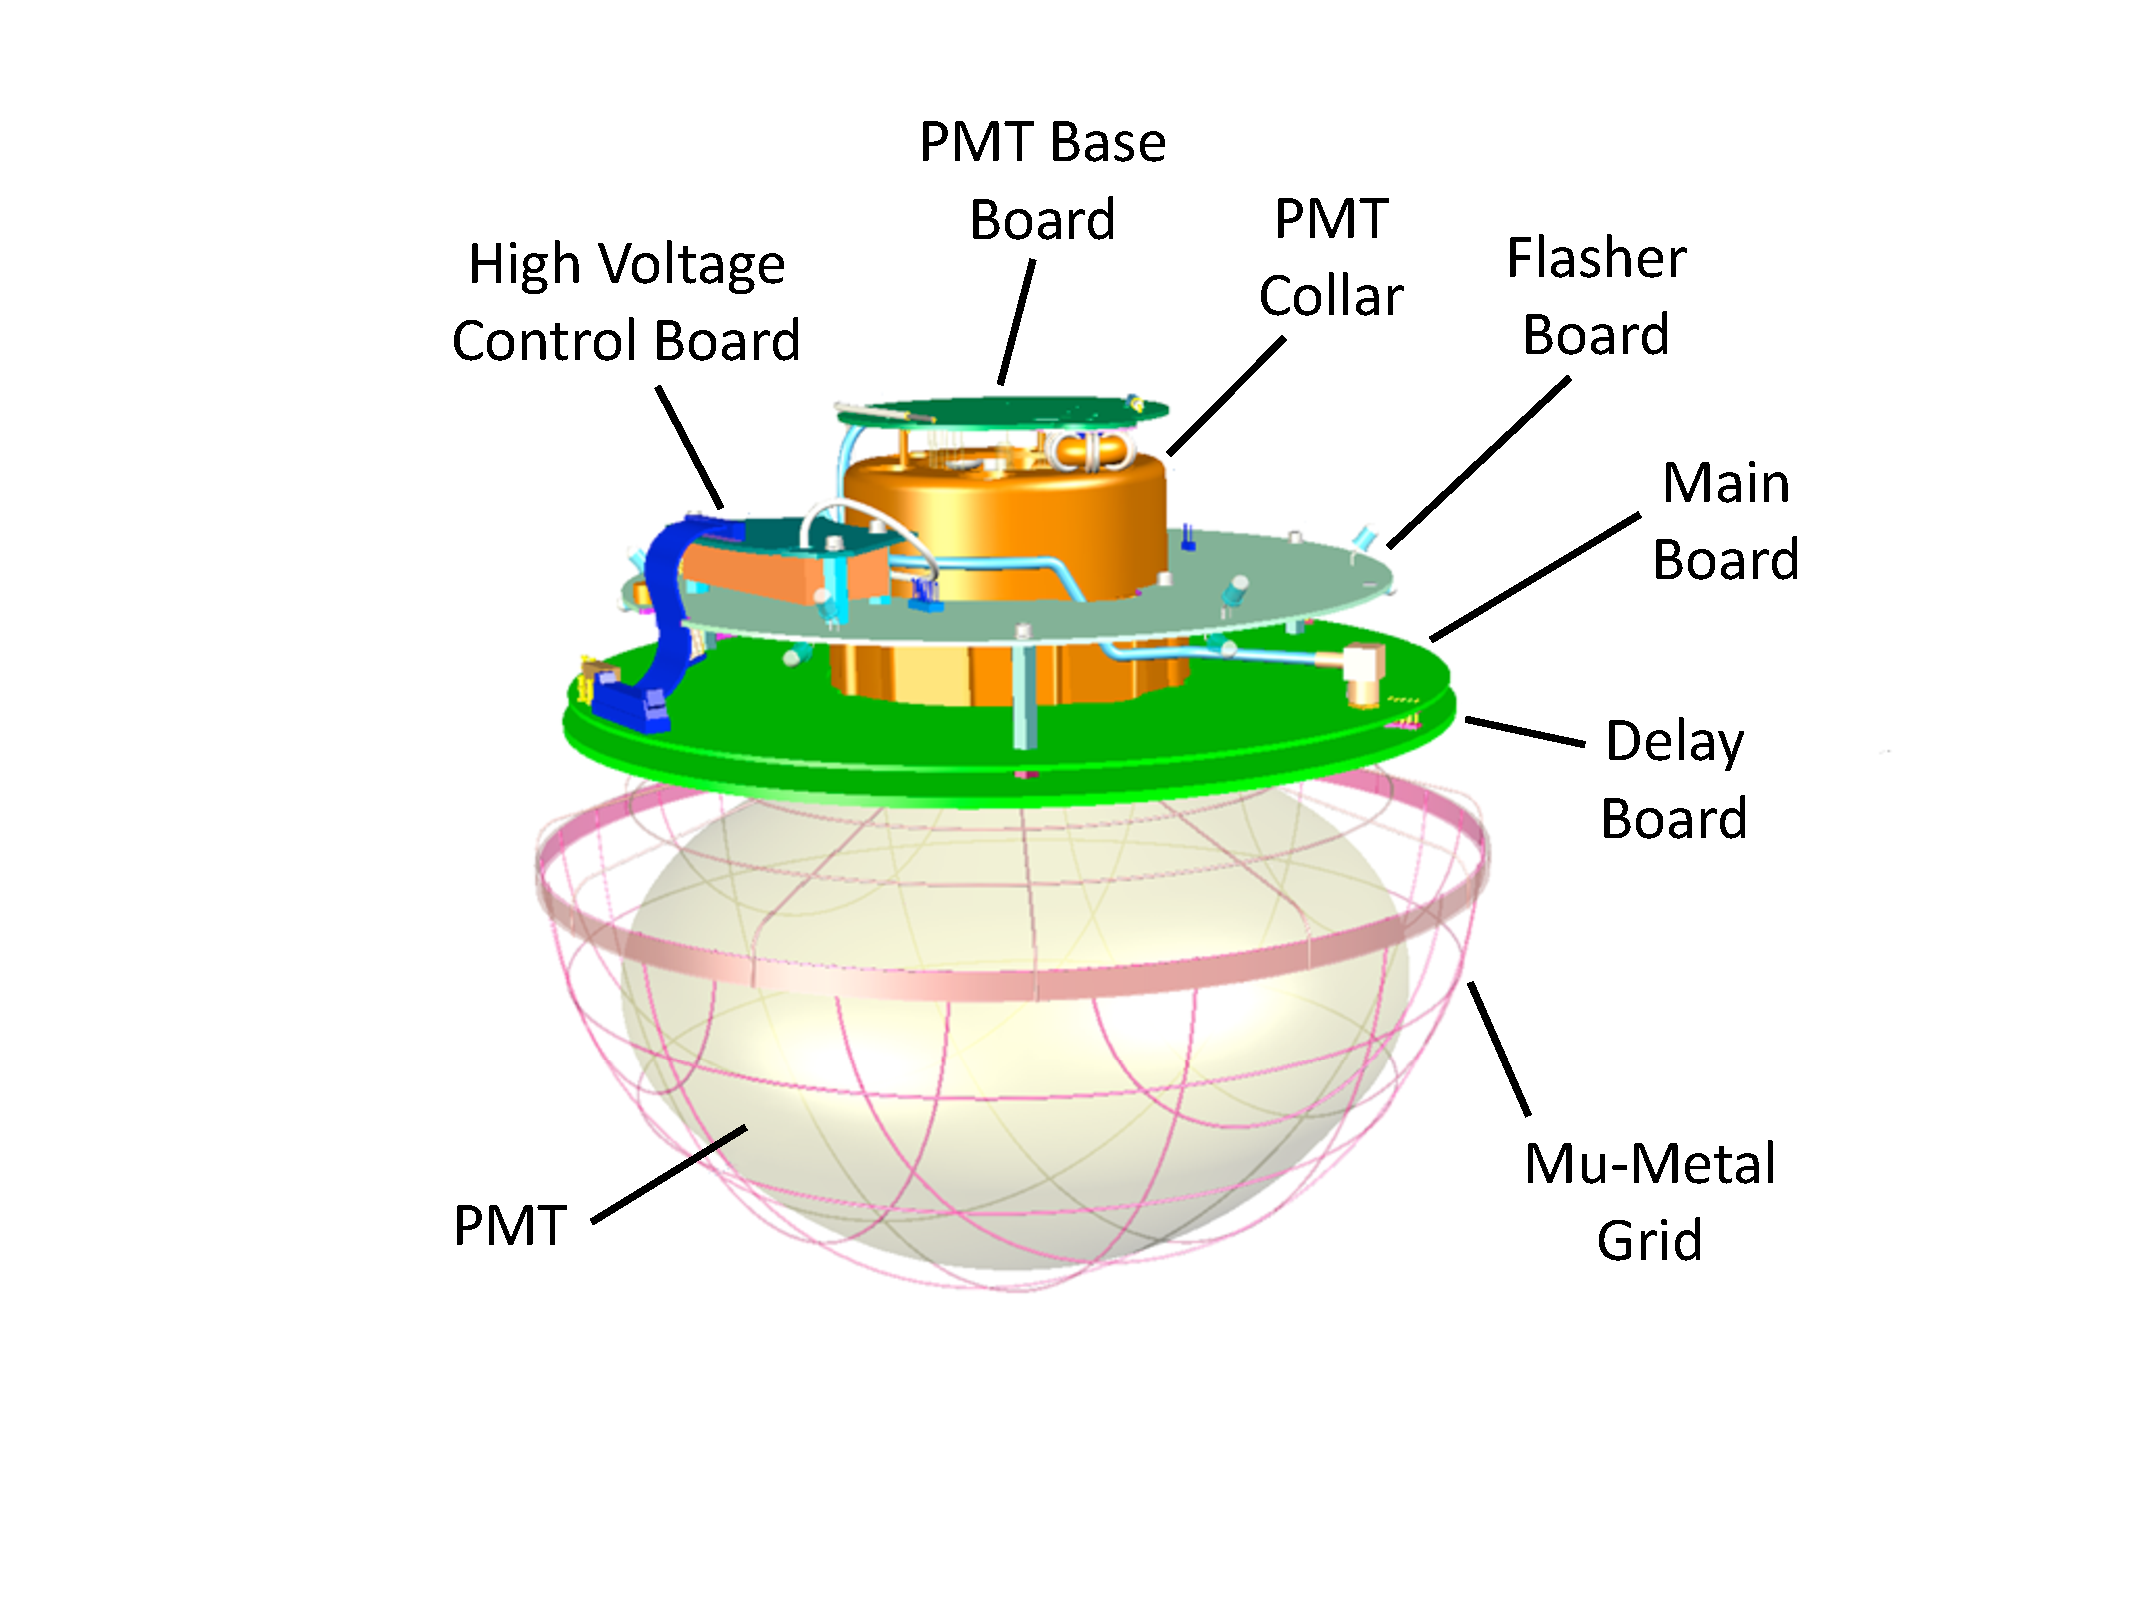
\includegraphics[width=\textwidth]{figures/icecube/domfig1a-DOM3DModel.pdf}
    \caption{Schematic of a DOM, taken from \cite{icecube_detector_17}.}
    \label{fig:dom-schematic}
\end{marginfigure}
\begin{marginfigure}
    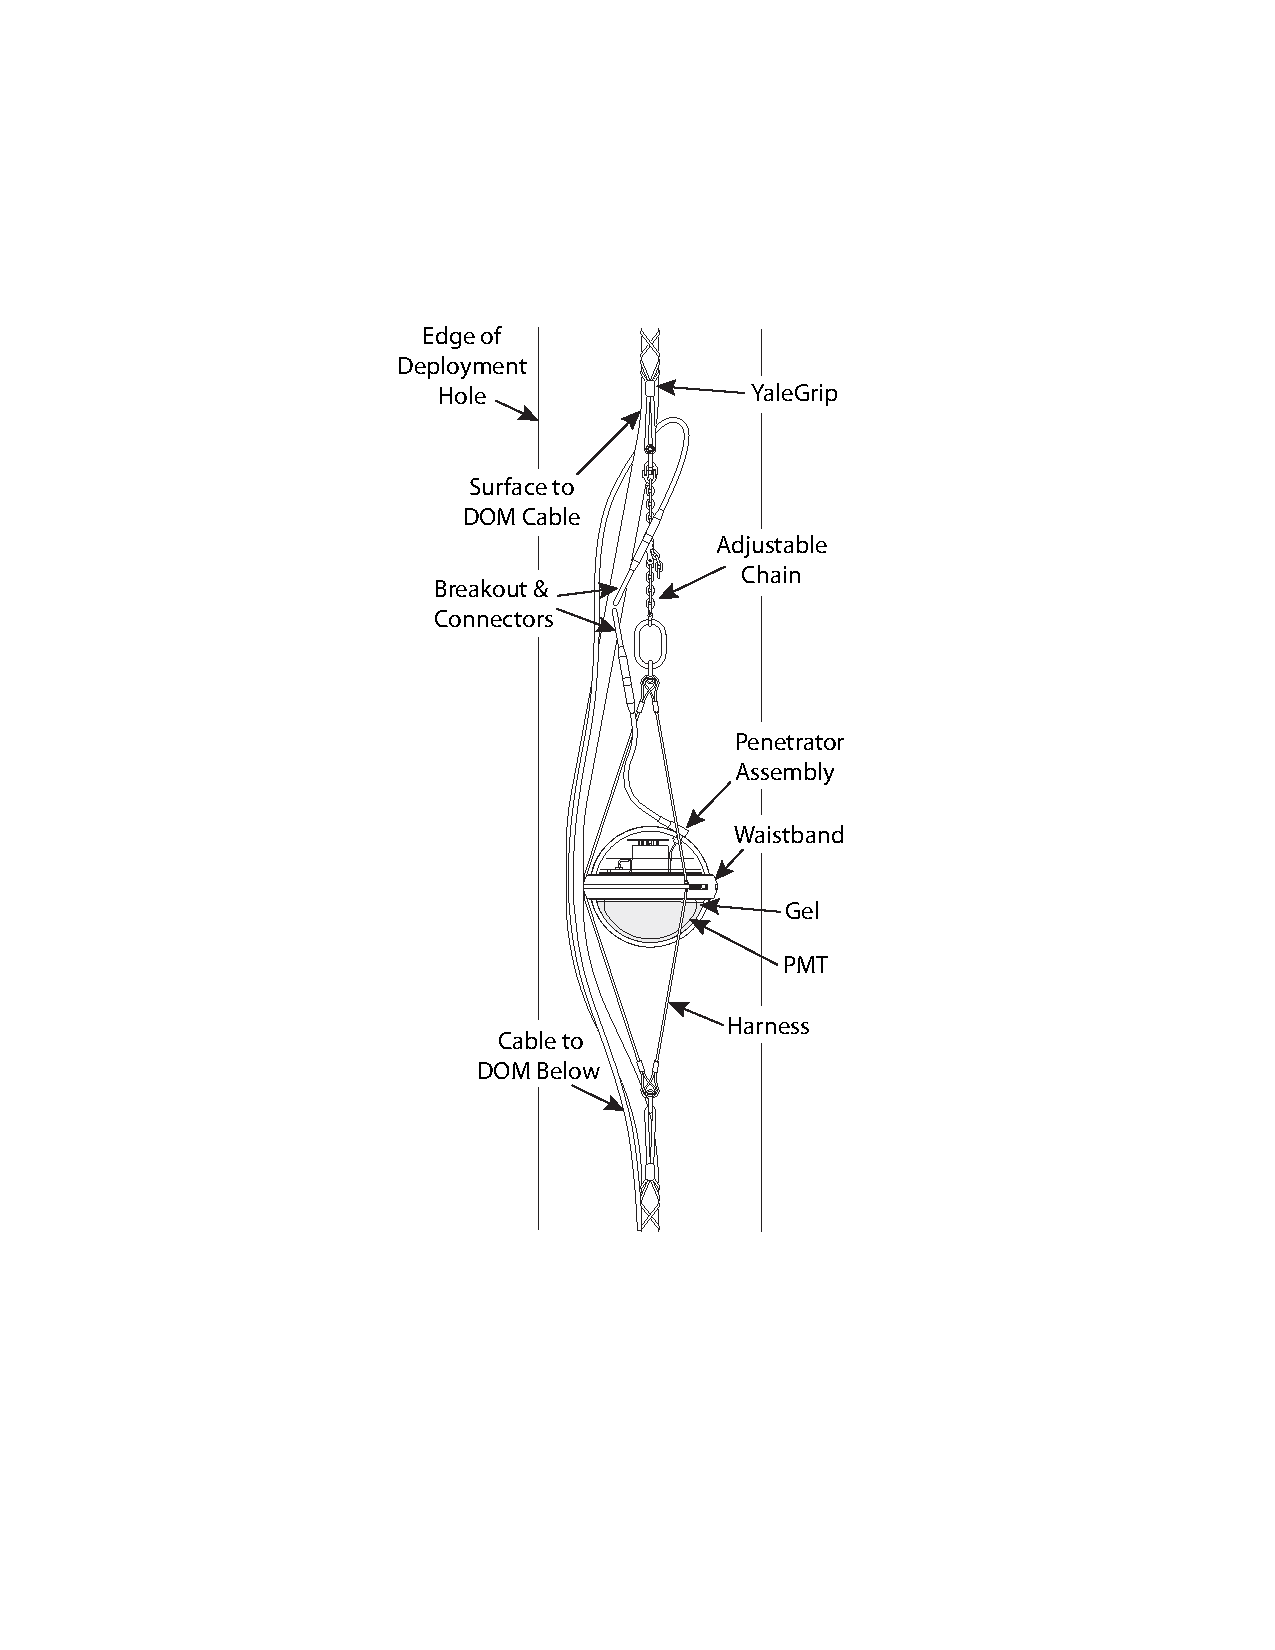
\includegraphics[width=\textwidth]{figures/icecube/domfig2a-CableAssembly.pdf}
    \caption{Schematic of the cable assembly of a DOM. Figure taken from \cite{icecube_detector_17}.}
    \label{fig:dom-cable-assembly}
\end{marginfigure}
The PMTs have a diameter of 10 inches and are sensitive to photons with wavelengths between 300~nm and 650~nm, with a maximum quantum efficiency of about 25\% at 390~nm.
Inside the DeepCore array, the peak efficiency reaches 34\%.
They are shielded from external magnetic fields with a mu-metal grid as shown in the schematic in Figure~\ref{fig:dom-schematic}.
The voltage at the PMT is measured and digitized by the on-board electronics\sidecite{icecube_daq} of the DOM in two separate readouts that are activated when the measured voltage rises above the equivalent of 0.25 photo-electrons (PE).
The first readout is the \emph{fast Analog-Digital Converter (fADC)} and measures the waveform continuously at a rate of 40~MHz.
The second readout, the \emph{Analog Transient Waveform Digitizer (ATWD)}, records the PMT voltage at a rate of 300~MHz in three channels with different gain levels to ensure that a large range\todo{what range?} of voltages can be recorded without saturation of the output.
The readout frequency of the ATWD is too high to be directly digitized and sent to the surface.
Instead, the ATWD voltage readout is buffered in 128 analog capacitors, corresponding to a readout time of $\sim$420~ns.
The buffered voltages are only digitized when at least one of the nearest or next-to-nearest DOMs on the same string also measures a signal within a 1~$\mu$s time window, which is referred to as the \emph{hard local coincidence (HLC)} condition.
The recorded waveforms are sent to the ICL on the surface, where they are compressed by applying the \emph{wavedeform} algorithm\sidecite{ic_spe_20}.
The output of this algorithm are reconstructed times and charges of single photo-electrons, which are taken as input by all further data processing steps described in section~\ref{sec:data-processing}.

The DOMs also contain a flasher board with 12 LEDs that can be used to emit pulsed light for the purpose of \emph{in-situ} detector calibration during special \emph{flasher runs} of the detector.
During such runs, the charge and time distributions of the observed pulses in the DOMs in response to the LED flashes are measured.
Since the light is emitted at known locations and at known times, the measured distributions allow inference on the absorption and scattering properties of the ice.
Because the total amplitude of the emitted light is less well known, this calibration method is less well suited for calibrating the total optical efficiency of the DOMs.
Instead, this property of the detector is calibrated more accurately from measurements of minimally-ionizing atmospheric muons, for which the energy loss is well known.
